The multiple asset test cases are designed to test the loss aggregation functions of the event-based risk calculator, such as:

\begin{itemize}
\item portfolio loss computation for a given ground motion field
\item calculation of portfolio loss exceedance curves
\end{itemize}

% ---------------------------------------------------------------------------
\subsubsection{Case 7a}
In addition to calculating individual asset and portfolio loss tables and exceedance curves, OpenQuake also calculates the insured losses and exceedance curves for individual assets and for the portfolio, if requested. Each loss type can be assigned a deductible and an insurance limit, specified in either relative or absolute terms with respect to the replacement value of the asset.

This purpose of this case is to test the computation of individual asset insured loss exceedance curves and the average insured loss for each asset.

Given an asset loss $loss$, and a deductible component of insurance $deductible$, and an insurance limit $limit$, the insured loss is zero if the asset loss is below the deductible. For losses above the deductible amount, insurance pays the difference up to the limit. The insured loss is thus the smaller of the difference and the insurance limit. The equation used for computing the insured loss is presented below:

\begin{equation}
	insured\_loss = min(max(loss - deductible, 0.0), limit - deductible)
\end{equation}

The insured asset losses are collected for each of the ground motion fields generated for the simulated stochastic event sets, and finally the exceedance curves for the insured losses are calculated.

The input models for this test case are based on those used earlier in the single asset test Case~1d. The deductible component of insurance is $0.1\times$ the cost of replacement of the asset. The insurance limit is capped at $0.8\times$ the cost of replacement of the asset.
% \begin{table}[htbp]

\centering
\begin{tabular}{ l r r r }

\hline
\rowcolor{anti-flashwhite}
\bf{Result} & \bf{Julia} & \bf{OpenQuake} & \bf{Difference}\\
\hline
Average asset loss & 44.50 &  & \% \\
Average asset insured loss & 11.46 &  & \% \\
\hline
\end{tabular}

\caption{Results for event based risk test case 7a}
\label{tab:result-ebr-7a}
\end{table}
% Table \ref{tab:result-ebr-7a} shows the comparison of the OpenQuake result for average annual loss with the expected result.

% ---------------------------------------------------------------------------
\subsubsection{Case 7b}
This case is designed to exercise the portfolio insured loss exceedance curve computation for an exposure model containing multiple assets. In this case, the vulnerability models of different assets of the same taxonomy are treated as uncorrelated. In OpenQuake, this can be specified in the job configuration file, by setting the value of the parameter `asset\_correlation' to zero.

The sampling of the loss ratios proceeds as described earlier in Case~6b, and the insured losses for the individual assets are obtained from the asset event loss tables as described in Case~7a. Apart from the individual asset insured loss exceedance curves, in this case, the portfolio insured loss exceedance curve is also computed. Finally, the average portfolio insured loss is computed as the area under the portfolio insured loss exceedance curve.
% \begin{table}[htbp]

\centering
\begin{tabular}{ l r r r }

\hline
\rowcolor{anti-flashwhite}
\bf{Result} & \bf{Julia} & \bf{OpenQuake} & \bf{Difference}\\
\hline
Average portfolio loss & 90.75 &  & \% \\
Average portfolio insured loss & 19.43 &  & \% \\
\hline
\end{tabular}

\caption{Results for event based risk test case 7b}
\label{tab:result-ebr-7b}
\end{table}
% Table \ref{tab:result-ebr-7b} shows the comparison of the OpenQuake result for average annual loss with the expected result.

% ---------------------------------------------------------------------------
\subsubsection{Case 7c}
This case is designed to test the computation of the individual asset loss curves, the portfolio loss exceedance curve, average asset losses, and the average portfolio loss, when the vulnerability models of different assets of the same taxonomy are treated as fully correlated. In OpenQuake, this can be specified in the job configuration file, by setting the value of the parameter `asset\_correlation' to one.

The list of assets and their taxonomies are shown in Table~\ref{tab:assets-tax1}. Table~\ref{tab:vf-ln-tax3-zcov} shows the mean loss ratios and corresponding coefficients of variation in the vulnerability function used in this test case.

Ground motion fields are generated for each of the ruptures generated in the 100,000 stochastic event sets as described in Case~7a and Case~7b. These ground motion fields are also used for the corresponding calculation in Julia.

Since the sampled loss ratios conditional on a given ground motion field for different assets of the same taxonomy are assumed to be fully correlated in this case, a single \emph{epsilon}, $\epsilon$,  is sampled from the standard normal distribution for each taxonomy. The parameters $m$ and $s$ from the vulnerability model are converted to the parameters $\mu$ and $\sigma$ of the corresponding normal distribution, and the sampled loss ratio is obtained simply as $\exp (\mu + \epsilon * \sigma)$.

The portfolio loss curve calculated using the implementation of the calculator in Julia is compared with that produced by OpenQuake in Figure~\ref{fig:lc-ebr-7c}. Only the aggregated results for the portfolio are shown here for brevity.

\begin{figure}[htbp]
\centering
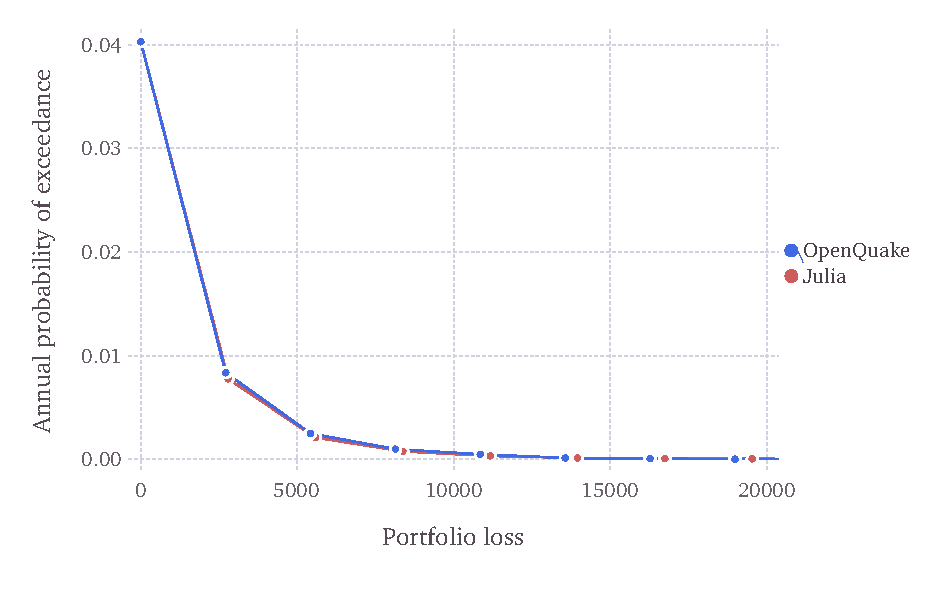
\includegraphics[width=12cm]{qareport/figures/fig-lc-ebr-7c}
\caption{Portfolio loss curve comparison for event based risk test case 7c}
\label{fig:lc-ebr-7c}
\end{figure}
% \begin{table}[htbp]

\centering
\begin{tabular}{ l r r r }

\hline
\rowcolor{anti-flashwhite}
\bf{Result} & \bf{Julia} & \bf{OpenQuake} & \bf{Difference}\\
\hline
Average portfolio loss & 88.10 &  & \% \\
Average portfolio insured loss & 18.87 &  & \% \\
\hline
\end{tabular}

\caption{Results for event based risk test case 7c}
\label{tab:result-ebr-7c}
\end{table}
% Table \ref{tab:result-ebr-7c} shows the comparison of the OpenQuake result for average annual loss with the expected result.

% ---------------------------------------------------------------------------